\subsection{Data}\label{subsec:data}
To achieve our goal, we opted for the public dataset ``Icons-50''~\cite{Icons50} , first introduced in~\cite{Hendrycks2018}.
According to the authors, this dataset was initially designed to test the robustness of classifiers to surface variations in objects.
The dataset includes both new styles of known objects and unexpected instances of known classes, and the authors propose two methods to improve the surface variation robustness of classifiers.

The Icons-50 dataset consists of 10,000 images belonging to 50 classes of icons (e.g., people, food, activities, places, objects, symbols, etc.) collected from different technology companies and platforms (e.g., Apple, Samsung, Google, Facebook, etc.).
Each class has icons with different styles (e.g., Microsoft's flat vector graphics icon style) and different class subtypes (e.g., `duck' or `eagle' subtypes in the `birds' class)~\cite{Icons50}.

To summarize, each entry in the dataset consists of the following parameters:
\begin{itemize}
    \item image - a 3x32x32 NumPy array corresponding to the RGB icon
    \item class - an integer between 0 and 49 representing the icon's class
    \item subtype - a string corresponding to the class subtype, e.g., ``broken\_heart'' for the class ``heart'' (label 26)
    \item style - a string corresponding to the icon's source, such as Microsoft or Apple
    \item rendition - an integer between 0 and 9 representing the icon's version
\end{itemize}

When analyzing the class distribution, we came to the conclusion that the Icons-50 dataset was considerably unbalanced, as seen in Fig.~\ref{fig:Icons50ClassDist}.

\begin{figure}[htbp]
    \centering
    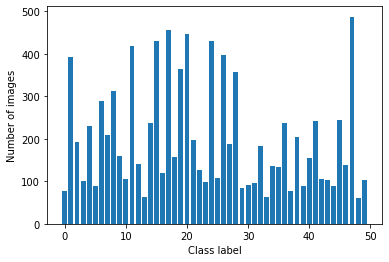
\includegraphics[width=0.48\textwidth]{images/icons50/class_dist}
    \caption{Class distribution of the Icons-50 dataset}
    \label{fig:Icons50ClassDist}
\end{figure}

This led to the creation of Icons-10, a subset of Icons-50 containing the top 10 most frequent classes in the dataset, with the old labels mapped to new values between 0 and 9.
The Icons-10 dataset comprises 4170 images and has a fairly balanced class distribution, seen both in Fig.~\ref{fig:Icons10ClassDist} , and in Table~\ref{tab:Icons10Desc}.

\begin{figure}[htbp]
    \centering
    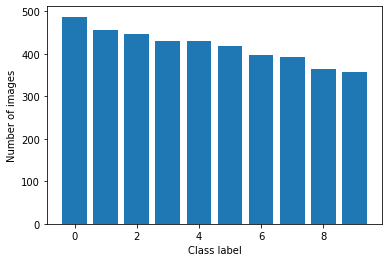
\includegraphics[width=0.48\textwidth]{images/icons10/class_dist}
    \caption{Class distribution of the Icons-10 dataset}
    \label{fig:Icons10ClassDist}
\end{figure}

\begin{table}[htbp]
    \centering
    \caption{Icons-10 Dataset}
    \begin{tabular}{cccc}
        \hline
        \textbf{Class} & \textbf{Old label} & \textbf{New label} & \textbf{No. samples} \\ \hline
        worker         & 47                 & 0                  & 487                  \\
        family         & 17                 & 1                  & 455                  \\
        flag           & 20                 & 2                  & 446                  \\
        face           & 15                 & 3                  & 429                  \\
        hands          & 24                 & 4                  & 429                  \\
        clock          & 11                 & 5                  & 417                  \\
        heart          & 26                 & 6                  & 396                  \\
        arrow          & 1                  & 7                  & 392                  \\
        cat            & 19                 & 8                  & 363                  \\
        ideograph      & 28                 & 9                  & 356                  \\ \hline
    \end{tabular}
    \label{tab:Icons10Desc}
\end{table}

\subsection{Methods}\label{subsec:methods}
We opted to adapt an already existing implementation of a cGAN model using the \texttt{keras} library, with the original source code available in~\cite{BrownleeCGAN, BrownleeGAN}.
In the original post, the author chooses to train the model with the MNIST Fashion dataset, which comprises gray-level images with 28x28 pixels, far different from the Icons-50 dataset specifications.

In the case of a regular GAN, in Fig.~\ref{fig:GANArch}, the generator takes in the input vector randomly drawn from the latent space and outputs the generated image, which is fed to the discriminator, alongside real examples from our dataset, and outputs a classification: whether it is real.

\begin{figure}[htbp]
    \centering
    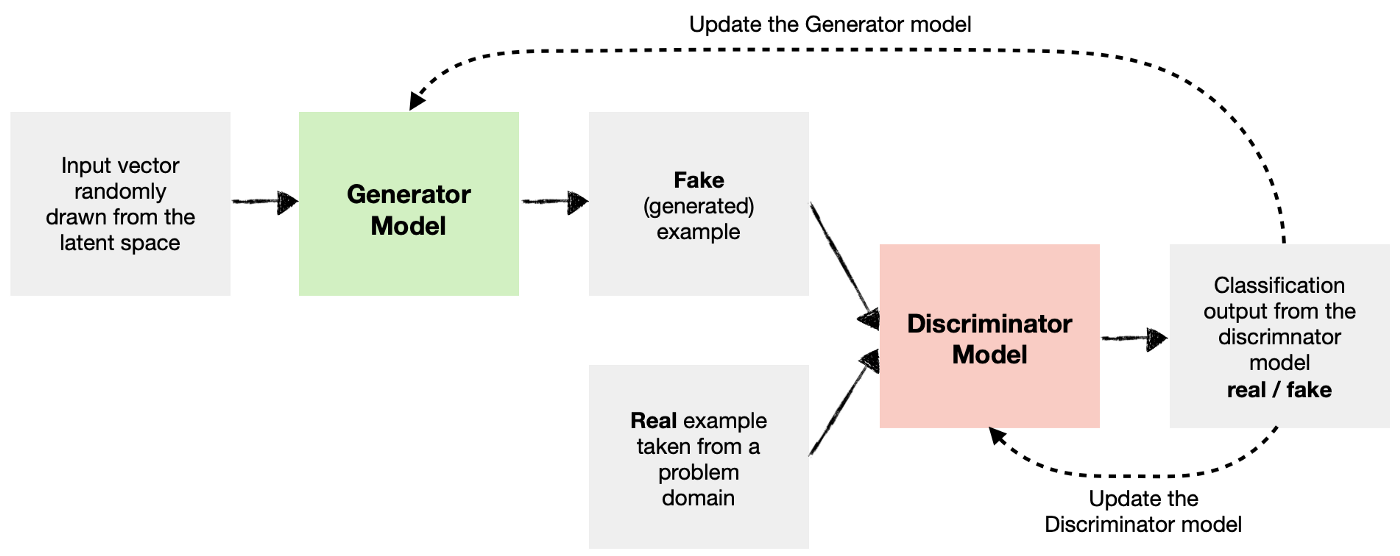
\includegraphics[width=0.48\textwidth]{images/architecture/gan_arch}
    \caption{Architecture of traditional Generative Adversarial Networks (GANs)}
    \label{fig:GANArch}
\end{figure}

The main difference between the regular GAN and the cGAN models can be seen in Fig.~\ref{fig:cGANArch}.
The conditioning variable, in our case, is the icon's class label, which is fed both to the generator when generating a new fake icon, and to the discriminator in order to learn whether it belongs to the specific class.

\begin{figure}[htbp]
    \centering
    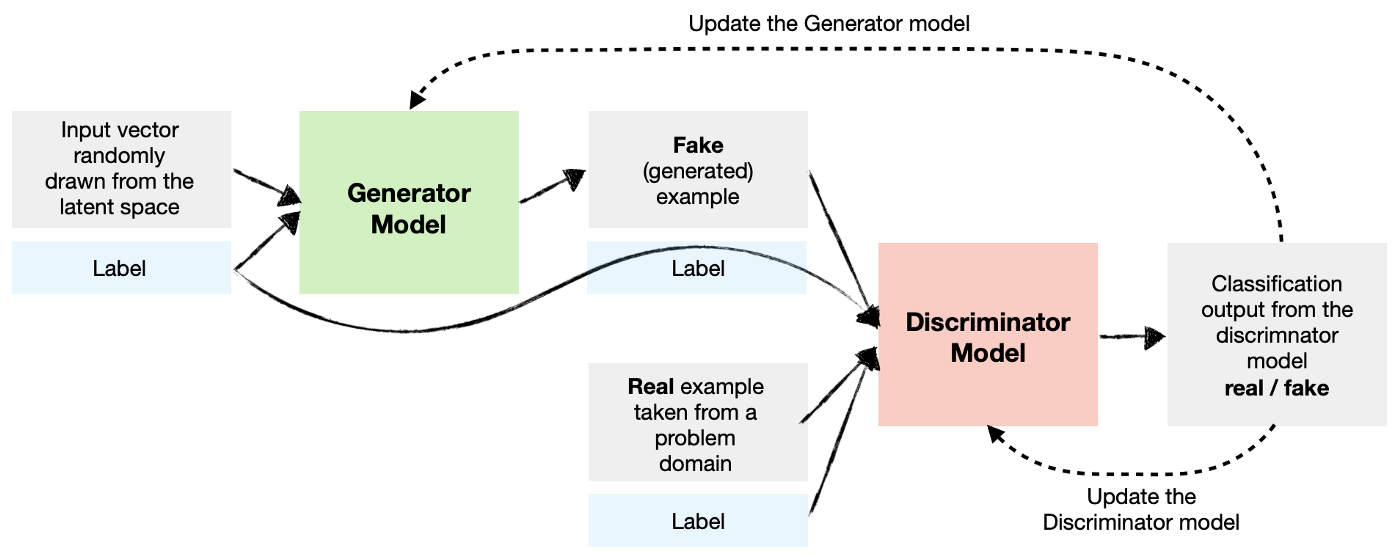
\includegraphics[width=0.48\textwidth]{images/architecture/cgan_arch}
    \caption{Architecture of Conditional Generative Adversarial Networks (cGANs)}
    \label{fig:cGANArch}
\end{figure}

With all this in mind, we built our model, starting with the generator.

As it is clear from Fig.~\ref{fig:GenStruct} , the generator takes in the class label of the icon we want to generate and an input vector drawn randomly from the latent space, with a dimension set at 100.
It has a total of 1.38M parameters.

In terms of the activation layers, we opted for the leaky RELU with an alpha of 0.2, apart from the output layer with a \textit{tanh} activation.

\begin{figure}[htbp]
    \centering
    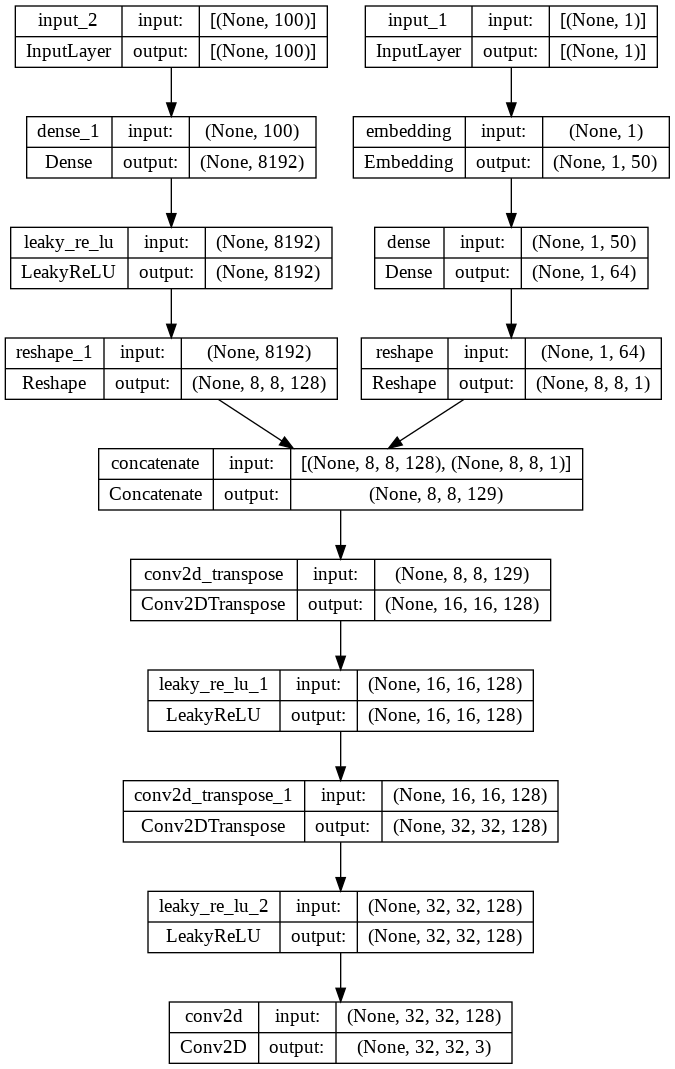
\includegraphics[width=0.4\textwidth]{images/summary/generator}
    \caption{Structure of the generator model}
    \label{fig:GenStruct}
\end{figure}

Now for the discriminator, as it is evident from (Fig.~\ref{fig:DiscStruct}), we again chose the leaky RELU function with an alpha of 0.2 for most of the model, apart from the output, which in this case has a \textit{sigmoid} activation, as we are dealing with a binary classification problem.

\begin{figure}[htbp]
    \centering
    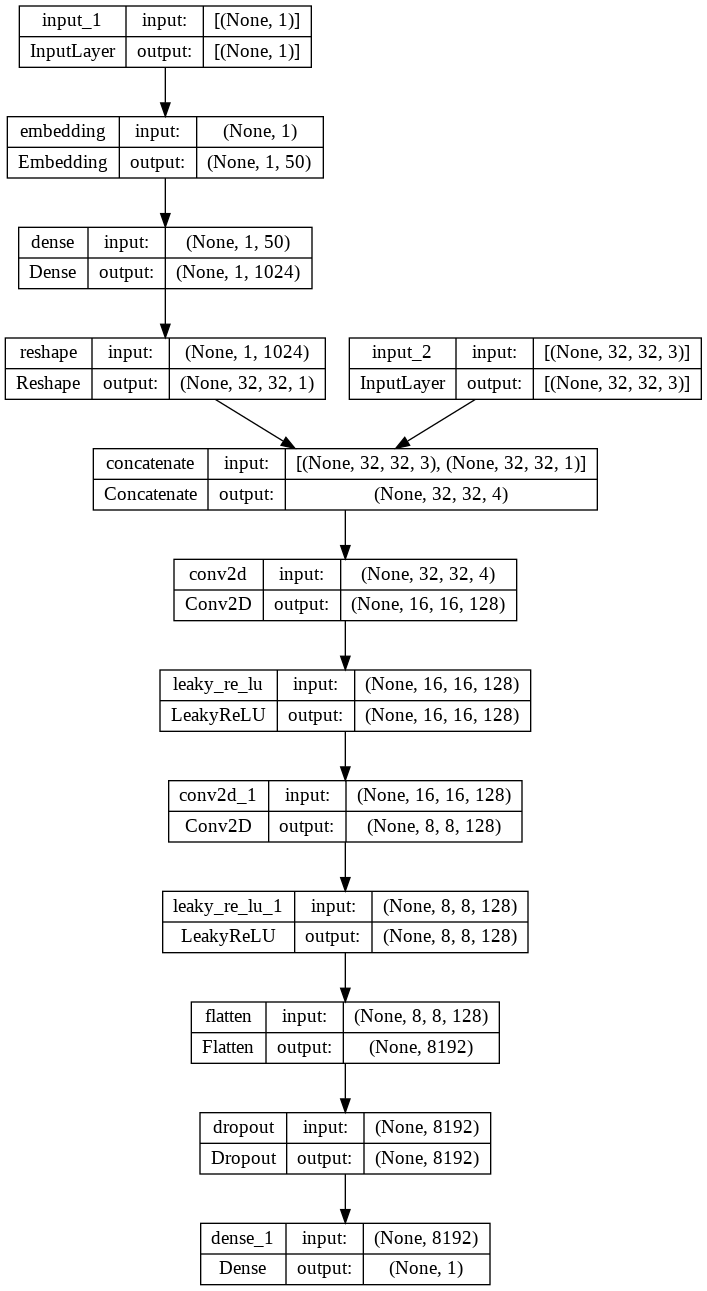
\includegraphics[width=0.4\textwidth]{images/summary/discriminator}
    \caption{Structure of the discriminator model}
    \label{fig:DiscStruct}
\end{figure}

Since the discriminator is to be trained individually, it must be compiled with a given optimizer, in this case, the Adam optimizer, with a learning rate $LR=\num{2e-4}$ and a $\beta_1=0.5$.
It has a total of 0.22M parameters.

Finally, we assemble our cGAN model by taking the generator's output and the input class label and feeding them to the discriminator, as seen in Fig.~\ref{fig:cGANStruct}.

\begin{figure}[htbp]
    \centering
    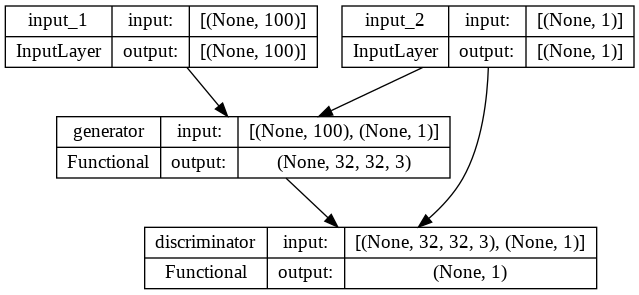
\includegraphics[width=0.48\textwidth]{images/summary/cgan}
    \caption{Structure of the cGAN model}
    \label{fig:cGANStruct}
\end{figure}

We chose to train trained two models with identical architectures, first with our original dataset, the Icons-50, and then with the new Icons-10 subset.
Given the smaller dataset, we picked an appropriate batch size to match its length, seen in Table~\ref{tab:ModelParams}.

\begin{table}[htbp]
    \centering
    \caption{Model parameters}
    \begin{tabular}{ccccc}
        \hline
        \textbf{Dataset} & \textbf{Parameters} & \textbf{Epochs} & \textbf{Batch Size} & \textbf{Latent Dim} \\ \hline
        Icons-50         & 1.6M                & 100             & 50                  & 100                 \\
        Icons-10         & 1.6M                & 100             & 30                  & 100                 \\ \hline
    \end{tabular}
    \label{tab:ModelParams}
\end{table}